\documentclass[fignum,nobf,man]{apa}
\usepackage{apacite}
\usepackage{bm}
\usepackage{pcl}
\usepackage{graphicx}
\usepackage{mathtools}
\usepackage[longnamesfirst]{natbib}
\usepackage[american]{babel}

\newcommand{\scN}[1]{$\times 10^{#1}$}

\rightheader{Bayesian Analysis for Systems Factorial Technology}
\shorttitle{Bayesian Analysis for Systems Factorial Technology}

\leftheader{Thiele \& Rouder}

\author{Jonathan E. Thiele and Jeffrey N. Rouder}

\title{Bayesian Analysis for Systems Factorial Technology}

\affiliation{University of Missouri}
\note{\begin{flushleft}

\vspace{1in}
Jeff Rouder\\
rouderj@missouri.edu
\end{flushleft}
}

\abstract{Systems factorial technology (Townsend and Nozawa, 1995) is a leading methodology for assessing the processing of multiple-feature items.  By using certain experimental designs and analyses, researchers can assess wether features are processed in serial, in parallel, or coactively.  Current practice is to assess the processing architecture of each individual, separately, as a fixed effects.  There is no way within the framework to combine results across people.  Conseuently,  the current approaches tend to overstate the evidence for heterogeneity of processing strategies across participants.  To address these shortcomings, we develop a series of hierarchical models that instantiate the processing architectures, and compare these models in light of data with Bayes factor.  Computations are performed via Savage Dickey density ratios with marginalization performed via MCMC sampling.  We report an application into Miller's (1956) notion of chunking.  We asked participants to compare object that are composed of separable features simultaneously, a perception task, and sequentially, a memory task.  We tested whether processing changed across the perception and memory tasks with the notion that participants might have to chunk features to store them, and that this chunking might make processing more efficient.  We found serial processing, however, for both perception and memory tasks.  We also find that given the resolution of the data in our studies, the best descriptions have a common processing strategy shared across all participants.  There was strong evidence against heterogeneity.}

\acknowledgements{Jeff Rouder, Department of
Psychological Sciences, 210 McAlester Hall, University of Missouri,
Columbia, MO 65211, rouderj@missouri.edu.  This research was
supported by National Science Foundation grants BCS-1240359 and SES-102408.}


\begin{document}
\maketitle

One of the key questions across cognitive psychology is the nature of latent processing that underlies various information-processing tasks.  Consider the perception of objects constructed of serveral features,  How these features are combined into coherent wholes remains timely and topical.  This question has generated a long and fruitful
mathematical-psychology literature on formal methods for understanding and querying processing architecture.  A selective list
includes \citet{Garner:Felfoldy:1970}, \citet{Liu:1996}, \citet{Schweikert:Townsend:1989}, \citet{Sternberg:1969}, \citet{Townsend:1990}, and \citet{Townsend:Ashby:1982}.   

\nocite{Townsend:Nozawa:1995}

To make the situation concrete, consider the stimuli presented in Figure~\ref{paradigm}.  We call these stimuli ``screwheads" because they resemble the top view of a flathead screw.  The stimuli are defined by two features: the size of the screwhead and the orientation of the slot.  The question is how these two features are processed. Perhaps the most common approach is to consider three different architectures:   1. {\em Serial processing}, where features are processed one-at-a-time in sequence; 2. {\em  Parallel processing}, where features are processed independently and simultaneously; and 3. {\em Coactive processing}, where the processing of one feature facilitates the processing of other features. 

The substantive question we address here is how different features are bound and held in working memory.  Perhaps the modal answer from \citet{Miller:1956} is that these features may be bound into one chunk rather than processed as two separate features.  There are several influential accounts of the role of working memory in chunking features together \citep{Atkinson:Shiffrin:1968,Cowan:1995,Mandler:1980}.  We ask whether this chunking changes the architecture of processing.  It may be that before chunking, items are processed serially, but afterwards, they are process in parallel or even co-actively.  

The approach we take to assess architecture is Townsend and Nozawa's (1995) {\em Systems  Factorial Technology}.   Systems factorial technology applies to a suite of approaches developed by Townsend and his students  \citep[see][for a review]{Townsend:Wenger:2004}.  The specific one used here is logical-rules variant \citep{Fific:etal:2008}.  Two key empirical results follow.  First,  simple objects with separable features seemingly are mediated by serial processing for most people \citep{Fific:etal:2010,Little:etal:2011}.  Second, the results are different for objects with integral features such color patches comprised of hue and saturation.   \citet{Little:etal:2013} show integral objects are seemingly mediated by coactive processing.  This combination of results, that separable features are processed serial but integrated features are processed coactively leads credence to the notion that the chunking of separable features in working memory may indeed change processing from serial to a more efficient form.  

Perhaps our most salient contribution here is methodological rather than substantive.  One of the limits of system factorial technology is that it is  applied to each participant individually.  Although this is certainly better than applying the method to aggregated data across all participants, the approach nonetheless treats each individual in isolation.  Results are usually tallies, say that 3 participants were better fit with a parallel model, 23 with a serial model, and 6 with a coactive model.  Unfortunately, any means of characterizing these results, generalizing to new participants, or comparing results across conditions is done outside the systems factorial inferential engine.  To address this limitation, we introduce a series of hierarchical models that instantiate various architectures.  Some of these models constrain all individuals to follow a common architecture though allow variability otherwise.  Models are compared through Bayes factor, an ideal approach  that follows directly from Bayes' rule.

In the next section we review system factorial technology. Included in this review is a discussion of the methodological limitations that motivate our Bayesian development.   Thereafter, we develop a set of hierarchical models and the derive Bayes factor computations for comparison among these models.  Then, we present two experiments to assess whether recalling information from working memory changes the architecture.  Each experiment consists of a perception condition and a memory condition, and the critical question is whether processing changes across these conditions.  The answer, perhaps surprisingly, is that it did not.  We observe signatures of serial processing across all conditions.
 
\section{System Factorial Technology}
We follow the logical rules approach to separating serial, parallel, and coactive processes described in \citet{Fific:etal:2010}:

%\subsection{Method}

{\bf Stimuli}.  The first step in applying systems factorial technology is operationalizing the features of a stimulus.  Consider the screwheads in Figure~\ref{paradigm}.  These stimuli have been used in several studies
in categorization \citep[e.g.,][]{Maddox:Ashby:1993,McKinley:Nosofsky:1995}
because the features, the size of the screw and the orientation of the slot, may be manipulated factorially.


\begin{figure}
\centering
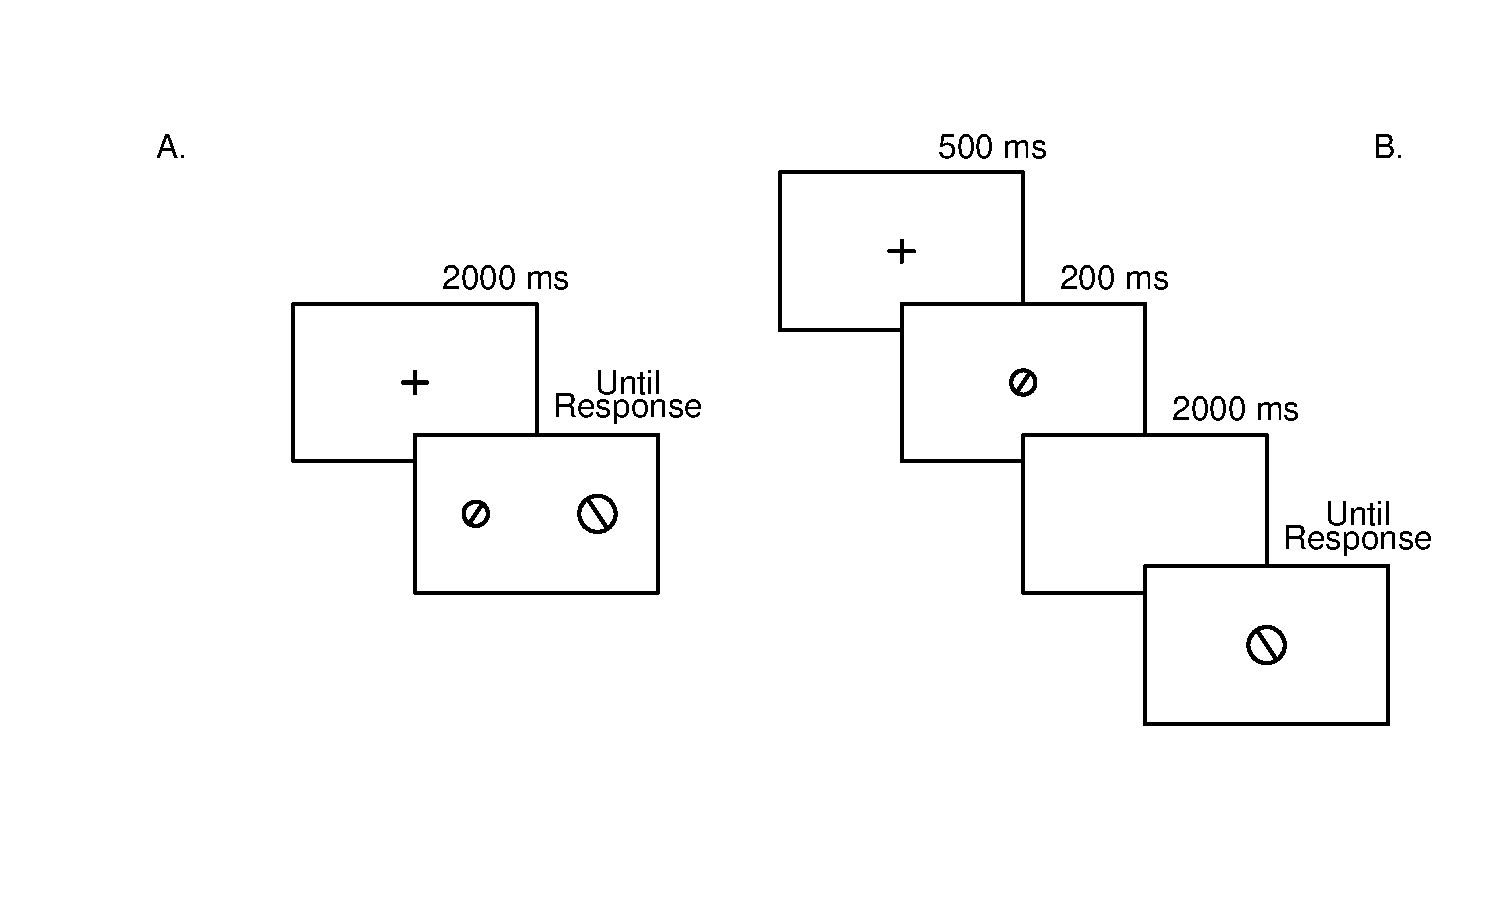
\includegraphics[width=6in]{experimentFrames.pdf}
\caption{Paradigm for Experiment~1.  {\bf A.} Schematic of trials in the perception task.  The participant decides if the screwheads differ in both radius and slot angle.  {\bf B.}  Schematic of trials in the memory task.}
\label{paradigm}
\end{figure}


{\bf Task}.  We asked participants to compare two screwheads (Figure~\ref{paradigm}A) and respond positive if the stimuli were different on both dimensions and negative otherwise.  There are three levels of difference on each features.  Consider orientation:  The two stimuli could have the same orientation, a small orientation difference, or a large orientation difference, and we denote these three levels as $0$, $1$, and $2$, respectively.  The same holds for radius: The two stimuli could have the same radius, a small radial difference, or a large radial difference, again denoted by $0$, $1$, and $2$, respectively.  Crossing these levels yield nine possibilities, and each possibility may be denoted by an ordered pair.   For example, the ordered pair $(0,2)$ denotes no change in orientation and a large change in radius across the pair of screwheads.  The task maps $(1,1)$, $(1,2)$, $(2,1)$, and $(2,2)$ into the positive response and the remaining 5 combinations into the negative response.  This mapping is shown in Table~\ref{task}.

\begin{table}
\caption{The Systems Factorial Task and Contrast}
\begin{tabular}{lccc}
& \multicolumn{3}{c}{Size}\\
Orientation &no change (0) & small change (1) & large change (2) \\ \hline
\multicolumn{4}{c}{Response Mapping}\\
no change (0) & - & - & - \\
small change (1) & - & + & + \\
large change (2) & - & + & + \\ \hline
\multicolumn{4}{c}{Cell Mean Notation}\\
no change (0) & $\bar{Y}_{00}$ & $\bar{Y}_{01}$ & $\bar{Y}_{02}$ \\
small change (1) & $\bar{Y}_{10}$ & $\bar{Y}_{11}$ & $\bar{Y}_{12}$ \\
large change (2) & $\bar{Y}_{20}$ & $\bar{Y}_{21}$ & $\bar{Y}_{22}$ \\ \hline
\multicolumn{4}{c}{Interaction Contrast}\\
no change (0) & 0 & 0 &0 \\
small change (1) & 0 & + & - \\
large change (2) & 0 & - & + \\ \hline
\end{tabular}
\label{task}
\end{table}


{\bf Analysis}.  The relevant data in the systems factorial method are the affirmative responses.  Let $Y_{11}$, $Y_{12}$, $Y_{21}$, $Y_{22}$ be distributions for the conditions $(1,1)$, $(1,2)$, $(2,1)$, and $(2,2)$, respectively, and let $\E(Y_{11})$, $\E(Y_{12})$, $\E(Y_{21})$, $\E(Y_{22})$ be the respective expectation value of these distributions.  Then the true mean interaction contrast (MIC), denoted $M$, is
\[
M = \frac{[\E(Y_{11})+\E(Y_{22})]-[\E(Y_{12})+E(Y_{21})]}{4}.
\]
The observed MIC is 
\[
\hat{M} = \frac{(\bar{Y}_{11}+\bar{Y}_{22})-(\bar{Y}_{12}+\bar{Y}_{21})}{4},
\]
where $\bar{Y}_{11}$, $\bar{Y}_{12}$ , $\bar{Y}_{21}$ , and $\bar{Y}_{22}$  denote the observed cell means for conditions $(1,1)$, $(1,2)$, $(2,1)$, and $(2,2)$, respectively.  The structure of these observed cell means and of the contrast is also shown in Table~\ref{task}.    The observed MIC is the best, unbiased estimator of the true MIC when the number of observations per cell is equal.
 
Perhaps \citet{Sternberg:1969} first popularized this interaction as a means of assessing architecture. \citet{Schweikert:1978} and \citet{Schweikert:Townsend:1989} provide more formal developments.  Townsend and Nozawa (1995) showed that the sign of $M$ is diagnostic of the nature of processing under certain technical conditions.  The key results we leverage here is as follows: {\bf 1.} If $M$ is negative, then processing is parallel.  {\bf 2.} If $M$ is positive, then processing is coactive.  {\bf 3.}  If $M=0$, then processing is serial.  The technical conditions are that RT distribution order with strength: $Y_{22} \leq Y_{21}$, $Y_{22} \leq Y_{12}$, $Y_{21} \leq Y_{11}$, and $Y_{12} \leq Y_{11}$.\footnote{The inequality of random variables refers to a stochastic ordering.  The statement $Y_{22} \leq Y_{21}$ is equivalent to the statement that $Pr(Y_{22}<t) \geq Pr(Y_{21}<t)$ for all $t$.}  In our experience, RT distributions seemingly always order with strength variable over ecologically valid ranges \citep[see ][]{Luce:1986}.  We know of no instances where this ordering has been violated with strength variables such as those used here, and we accept these technical conditions as assumptions without further confirmation.

\subsection{The Methodological Limitation}
A conventional approach is to assess the interaction contrast
separately for each individual.  Figure~\ref{surf1}B provides an example.  Here we have plotted the contrast with 80\% confidence intervals for each individual's MIC.  As can be seen, 22 of the 32 of the confidence intervals
contain 0, 5 of the 32 are localized above zero, and 5 of the 32 are localized below
zero.  One interpretation is that 22, 5, and 5 of the participants provide
support for serial, parallel, and coactive architectures,
respectively. 

\begin{figure}
\centering
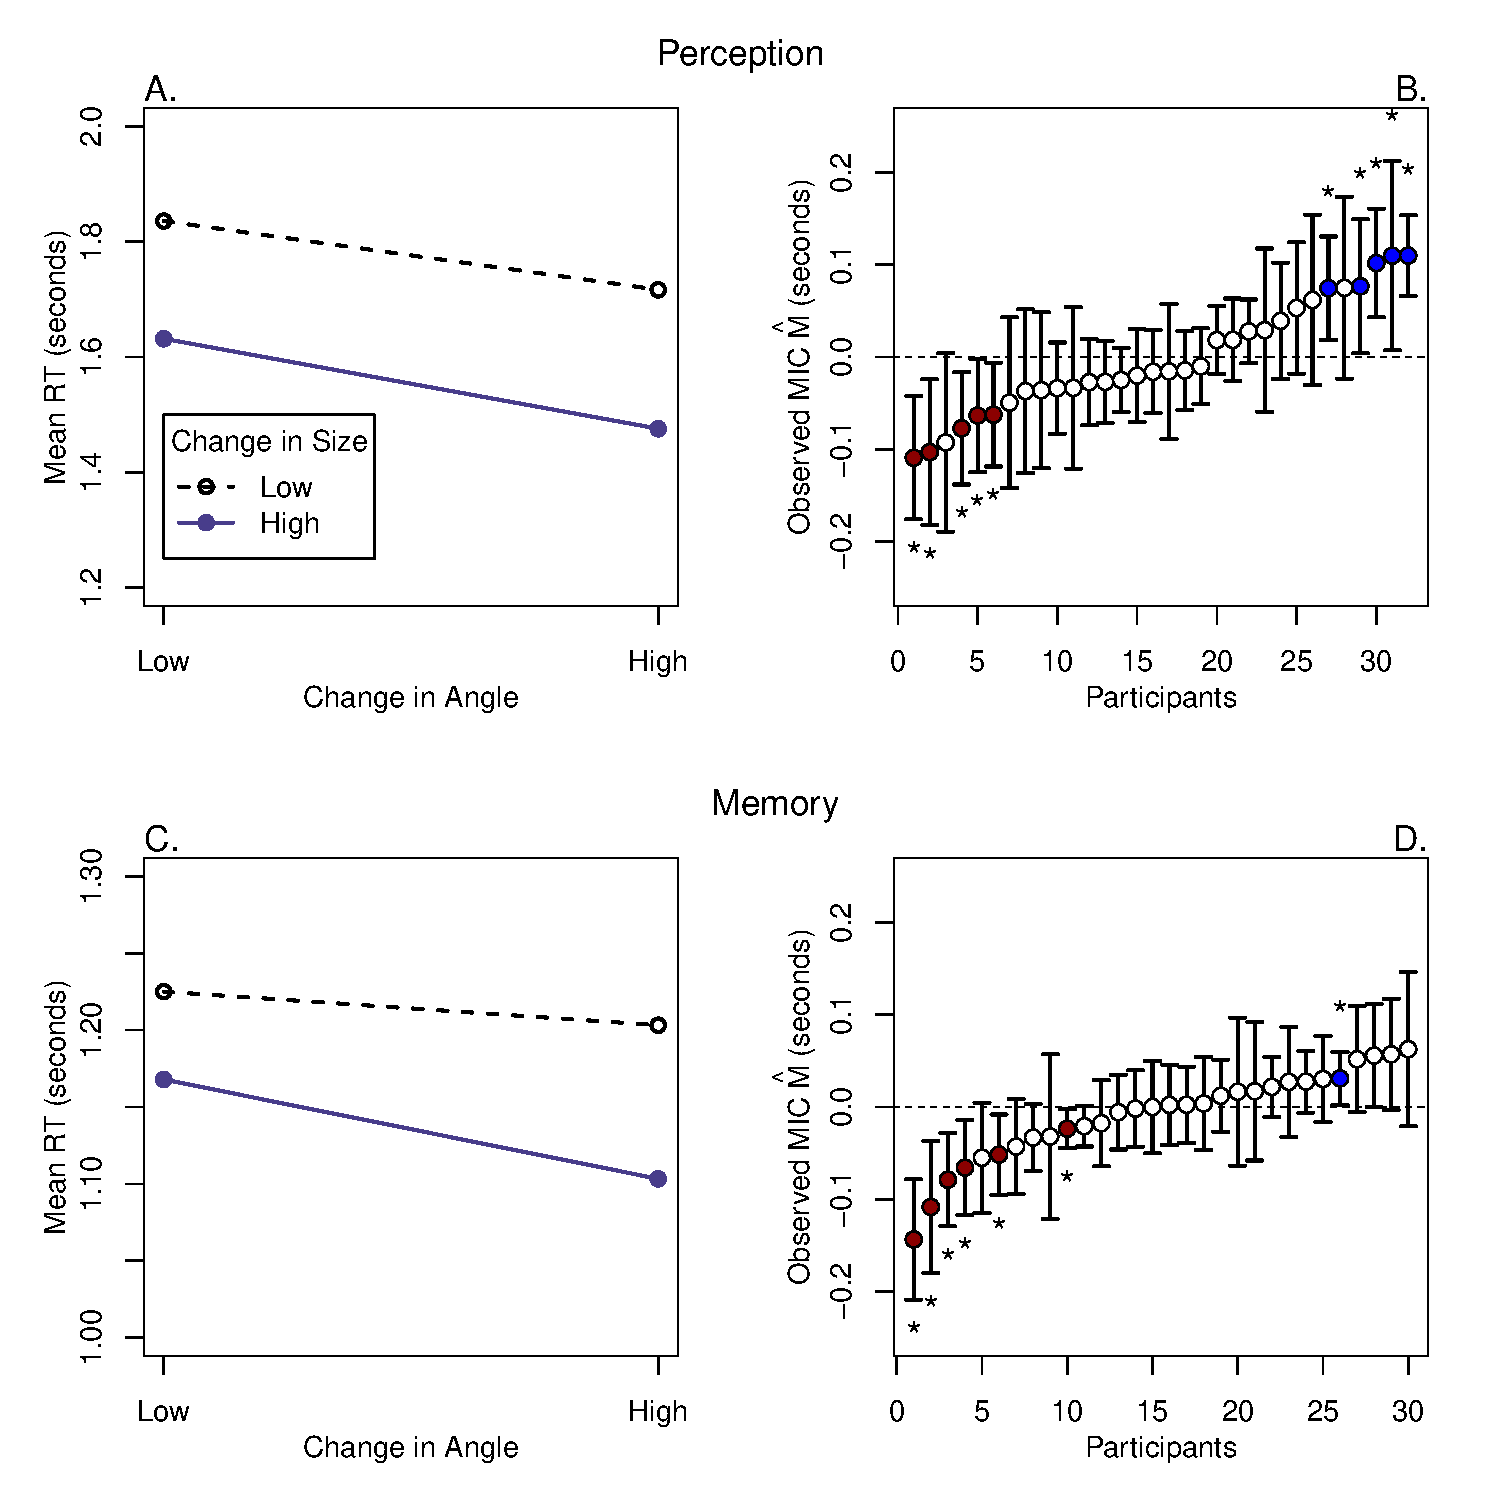
\includegraphics[width=6in]{jonFigures/jE1.pdf}
\caption{Results from Experiment 1:  {\bf A.,C.} Observed mean response times for Experiments 1A (perception) and 1B (memory), respectively.  {\bf B., D.} Observed mean interaction contrasts (MICs) with 80\% confidence intervals for each if 31 individuals.  The CIs with open circles contain zero (serial processing); those with darkened circles and an asterisk below are all negative (parallel processing); those with darkened circles and an asterisk above are all positive (coactive processing).}
\label{surf1}
\end{figure}

We think there are two main problems with this approach:
\begin{itemize}

\item There is a difficult asymmetry where the serial signature is a point hypothesis while the parallel and coactive signatures are hypotheses across respective halves of the real line.  The usual significance test approach allows rejection of the point but not acceptance of it.   The usual approach of holding the Type I error rate constant is not appropriate here because it privileges serial processing.  Even more problematic, this privilege varies with sample size, and it is almost complete with  small sample sizes where Type II errors are common.  To address this issue, we chose 80\% threshold on
the confidence interval.  Yet, such a choice plays an outsized in classifying individuals' architectures.  

\item There is an inherent bias toward concluding that processing architecture varies across individuals.  In fact, this conclusion is virtually guaranteed from sample noise considerations alone.  If each participant uses a serial process, for example, then we will reject seriality with fixed probabilities.  The situation is worse if parallel or coactive architectures hold.  Because we have limited samples per individual, the limited resolution of individual-by-individual testing will  lead to many participants being misclassified and the appearance of heterogeneity. 
\end{itemize}

This last point about whether or not people use different
architectures is crucial.  If they do not, that is that everyone or
at least a sizable majority of people use the same architecture, then
this invariance serves as a primitive of processing.  Questions that
follow naturally are about which tasks are served by which
architectures, and such correspondences become targets to be explained
by theory.  Alternatively, if people do vary in choice of architecture
even for the same task, then the focus shifts to which people use
which architectures, perhaps with measures of skills and personality
serving as predictors.  We think it is wisest to not presuppose an
answer to this question.  Yet, unfortunately, the available
methodologies are seemingly biased toward individual differences
because each participant is assessed independently and separately.


\section{Model Specification}

To address the limitations in the current approach,
we develop a set of hierarchical models that allow for the pooling of
information across participants.  We do so in the Bayesian framework
and use Bayes factor model comparison to draw inferences.  This
approach addresses the previous two limitations.  First, though there are critical specifications, these are made
transparently as an expectation about interaction effects.  Second, it is possible to specify models where all participants follow a common architecture.  For example, we can construct a model where all participants are parallel.  These common architecture models can be compared and they may be compared to models where individuals may vary in architecture.  

%We develop two separate sets of mixed parametric models of response
%time to assess the interaction contrast.  The first set is based on
%the normal distribution, and the advantages are two-fold: (a) the
%normal is computationally convenient in this application leading to
%rapid model development, and (b) the MIC is easily parameterized and
%the placement of constraint, say that MIC must be positive, is
%straightforward to implement.  These advantages are substantial, yet
%they are at least partially offset by the obvious misspecification of
%the normal for RT.  The misspecification is two-fold: (a) RT is skewed
%rather than symmetric, and (b) condition effects tend to manifest as
%multipliers or scale factors rather than as addends or shifts \cite{Wagenmakers:Brown:2007,Luce:1986,Rouder:etal:2010d}.  To account for these misspecification we developed a
%separate gamma-distributed line of models where condition effects are
%manifest on the scale parameter.  Unfortunately, while scale models
%are entirely appropriate for RT, they are not well suited for
%assessing MICs.  We provide a work-around where scale factors add
%instead of multiply.  Yet, this work-around is awkward, as discussed
%subsequently.

We develop a set of mixed models of response time to assess the interaction contrast.  Let $Y_{ijk\ell}$ be the $\ell$th response time for the $i$th participant in the $j$th level of Factor A and the $k$th level of Factor B, $i=1,\ldots,I$, $j=1,2$, $k=1,2$, and $\ell=1,\ldots,L_{ijk}$:
\begin{eq}
Y_{ijk\ell} \sim \mbox{Normal}\left(\mu_{ijk},\sigma^2\right),
\end{eq}
The cell mean parameters $\mu$ are additively decomposed as
\begin{eq}
\mu_{ijk} = \eta_i + \alpha_{i}s(j)+ \beta_{i}s(k) + \gamma_i s(j)s(k),
\end{eq}
where $s(m) =(-1)^m$ for $m=1,2$.   The parameters $\eta_i$, $\alpha_i$, $\beta_i$, $\gamma_i$ describe
 each participant's grand mean, main effect for Factor A, main effect
 for factor B, and interaction, respectively.    The function $s$ is a compact means of imposing the usual sums-to-zero, balance constraints so that main effects are defined as balanced differences from the grand means and that interactions are defined as balanced differences from main effects.   This parameterization is similar to classic ANOVA parameterizations.  The difference is in the treatment of individual.  Note here that there are separate grand mean, main effect, and interaction parameters for each individual, which is a different than the usual within-subjects formulation. 
 
The advantages of the above specification are two-fold: (a) the normal is computationally convenient in this application leading to rapid model development and quick converging chains, and (b) the MIC is easily parameterized and the placement of constraint, say that MIC must be positive, is straightforward to implement.  These advantages are substantial, yet they are at least partially offset by the obvious misspecification of the normal for RT.  The misspecification is two-fold: (a) RT is skewed rather than symmetric, and (b) condition effects tend to manifest as multipliers or scale factors rather than as addends or shifts \citep{Wagenmakers:Brown:2007,Luce:1986,Rouder:etal:2010d}.   One approach to address this misspecification is the development of models with three-parameter shift-scale-shape skewed distributional forms such as the Wiebull or lognormal.  We have had success with these forms in the past \citep{Rouder:etal:2005a,Rouder:etal:2008d, Rouder:etal:2010d,Rouder:etal:2015}, but development here is problematic.  The main hurdle is characterizing the sign of the interaction in scale models.  For instance, how can the multiplicative model on scale parameters across produce the null interaction contrast that corresponds to serial processing.   In light of these difficulties, we develop the normal base model here.  


With this normal specification, $M_i$, the true interaction contrast, is
\[
M_i =\gamma_i
\]

The serial architecture is straightforwardly implemented by placing the following constraints on  $\gamma_i$:
\begin{eqa}
\mbox{Serial:} && \gamma_i=0.
\end{eqa}

Parallel models imply that each $\gamma_i<0$.  We implement this
constraint in two ways:
\begin{eqa}
\mbox{Parallel-1:}&& \gamma_i \sim \mbox{Normal}_-(\nu_\gamma,\delta_\gamma)\\
\mbox{Parallel-2}&& \gamma_i=\gamma_0, \;\;\gamma_0<0,
\end{eqa}
where $\mbox{Normal}_-$ denotes a negative half-normal distribution.
In the first specification, each participant has their own unique
interaction parameter, and all of these parameters are constrained to
be negative.  In the second specification, all participants share a
common, constant interaction parameter which is constrained to be
negative.  The first specification is far more flexible and allows for
individual variation.  The second is far more compact with a model
dimensionality of a single parameter rather than $I$ parameters.
Parallel-2 may be a preferred description when there are not
sufficient observations per participant to resolve true participant
effects.  Moreover, the parallel-2 model is comparable in parsimony to the serial model in that there is no individual variability in either specification.

Coactive models imply that each $\gamma_i>0$ which was implemented as 
\begin{eqa}
\mbox{Coactive-1:}&& \gamma_i \sim \mbox{Normal}_+(\nu_\gamma,\delta_\gamma)\\
\mbox{Coactive-2:}&& \gamma_i=\gamma_0,\;\;\gamma_0>0.
\end{eqa}
As with parallel models, the first specification captures individual differences in the interaction while the second specification does not.

In these models, all participants share a common architecture; that
is, either everyone displays serial processing, everyone displays
parallel processing, or everyone displays coactive processing.  These
models are parsimonious in that they do not specify differences across
people allowing for a straightforward interpretation and easy generalization.

Although we are excited about the above models that specify a common architecture across all people, it may be that people truly vary.  Some might truly perform the task inserial; others might truly perform the task in parallel, and still others might truly perform the task coactively.   To account for
this possibility, we included a general model
\begin{eqa}
\mbox{General:} && \gamma_i \sim \mbox{Normal}(\nu_\gamma,\delta_\gamma).
\end{eqa}  
There are no constraints on $\gamma_i$ other than the parametric shape specification.

Bayesian analysis proceeds with specification of priors on all parameters.  It is useful to think in terms of two classes of parameter: those whose specification is common across all models under consideration, and those whose specification varies to reflect the different processing architecture.  The common parameters are $\sigma^2$, $\bfeta$,  $\bfalpha$, and $\bfbeta$, and because these parameters serve in common, the prior settings do not materially affect estimates or Bayes factor model comparison statistics.  These priors are provided in the Appendix.  The more critical prior specifications are those on $\bfgamma$, the interaction parameters.

There are two constant-effect models, parallel-2 and coactive-2, and prior is needed in each for $\gamma_0$, the constant interaction among all participants.  For parallel-1, we chose $\gamma_0 \sim \mbox{Normal}_-(0,.1^2)$; for co-active-1, we chose $\gamma_0 \sim \mbox{Normal}_+(0,.1^2)$, where all values are specificed in seconds.   This prior for the coactive-1 model is shown in Figure~\ref{gammPrior}A.  Interactions tend to be small, but values as large as .3 s are plausible.  We view these specifications as reasonable because impossibly large interactions do not lower the marginal probability of data under the model.

The models with separate individual effects. parallel-1, coactive-1, and the general model requires placing models on $\nu_\gamma$ and $\delta_\gamma$, the population-level parameters.  We chose
\begin{eqa}
\nu_\gamma &\sim& \mbox{Normal}(0,.01^2)\\
\delta_\gamma &\sim& \mbox{Inverse Gamma}(3,.02)
\end{eqa}
These values were picked values so that the marginal prior distributions on each $\gamma_i$ were spread within a
range of a few hundred milliseconds while there was little prior covariation among individuals.  Figure~\ref{gammPrior}A shows the bivariate distributions for two such $\gamma_i$ for the general model.  Hence, while small individual effects are likely, larger ones are not {\em a priori} implausible.   Appropriately truncated versions of these hierarchical normal priors were placed on $\gamma$ for the parallel-1 and coactive-1 models.   

\begin{figure}
\centering
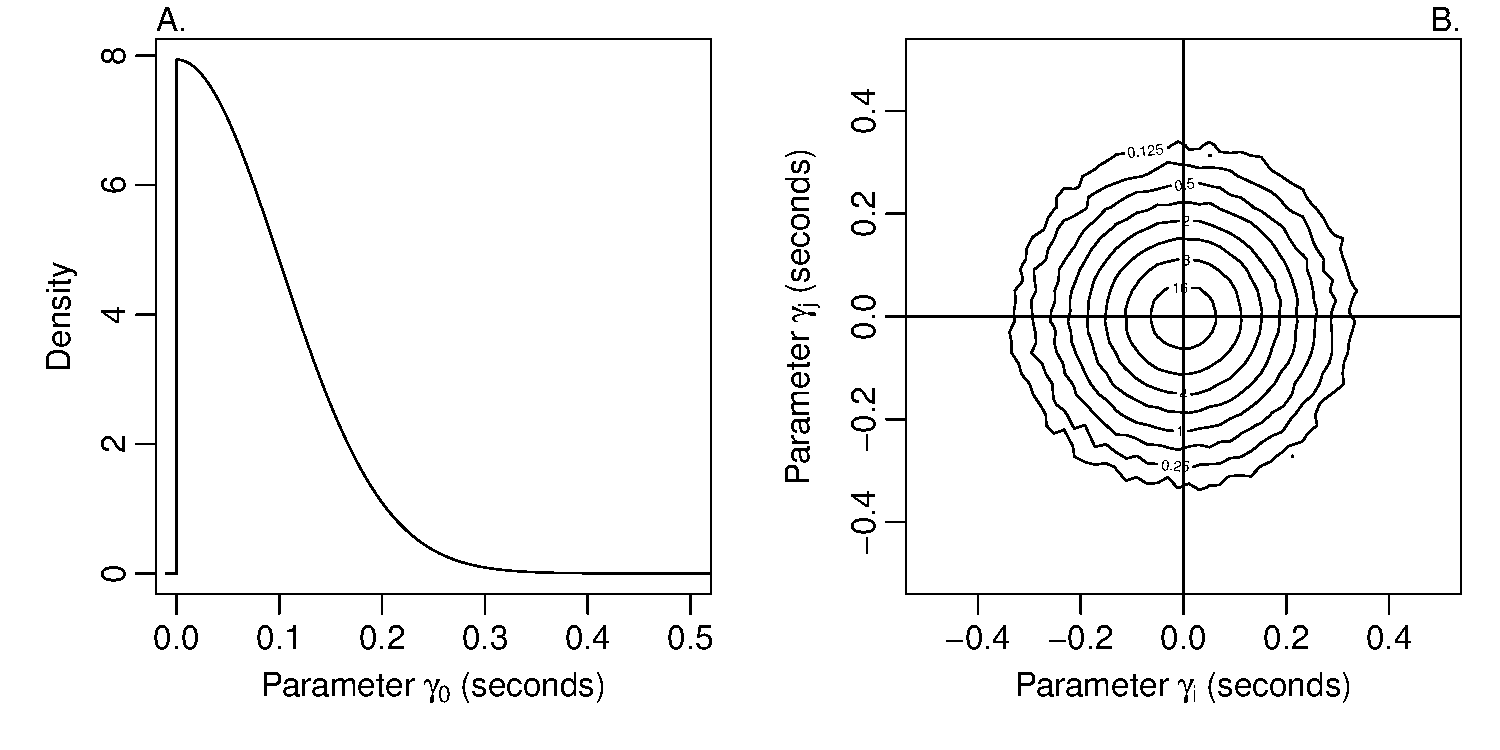
\includegraphics[width=6.5in]{gammaPriors.pdf}
\caption{Prior specification of interaction parameters $\bfgamma$.  {\bf A.} The bivariate distribution of interactions across any two participants for the general model.  Coactive and parallel models are specified by trunctating this distribution to the first and third quadrants, respectively.  {\bf B.} The univariate distribution of interaction for the coactive model with a common interaction term across people.}
\label{gammPrior}
\end{figure}



%\subsection{Gamma Model Specification}
%The key parametric specification in the above development is that
%response times follow a normal distribution with constant variance
%across conditions.  Yet, it is well known that RTs are skewed and that the standard deviation increases with the
%mean \citep{Luce:1986,Rouder:etal:2010d,Wagenmakers:Brown:2007}.  These facts motivated a second
%line of development with gamma-distributed models.  We used a gamma distribution with a shape parameter fixed to 2.0, or the shape of two exponentials added together.  There were two free parameter, the shift and scale,  denoted
%$\psi$, $\theta$.  The probability density
%function is:
%\[
%f(y;\psi,\theta) = \frac{1}{\theta}\left(\frac{y-\psi}{\theta}\right)\exp\left(-\frac{y-\psi}{\theta}\right)
%\]
%
%The data model is
%\begin{eq}
%Y_{ijk\ell} \sim \mbox{Gamma}\left(\psi_i,\theta_{ijk}\right).
%\end{eq}
%In this specification, shift parameters vary across people but not
%conditions.  This lack of dependence of shift on condition is fairly common, and the conventional interpretation is that the shift latency is nuisance variation from  motor and encoding processes rather than from cognitive
%processes \citep{Ratcliff:1978}.  Scale parameters, which reflect the speed of cognitive processes, depend on people
%and conditions.  These scale parameters are the target of inquiry.
%
%Ideally, one would place a multiplicative model on scale to insure that scale values are always positive \citep{Rouder:etal:2005a}.  Yet, this proved intractable in the current context because there is no specification that would leave the interaction contrast $M_i$ to be identically zero.  As an alternative, we placed  a rather awkward additive model on the scale parameter:
%\begin{eq}
%\theta_{ijk} = \eta_i + \alpha_{i}s(j)+ \beta_{i}s(k) + \gamma_i s(j)s(k).
%\end{eq}
%With this specification, 
%\[
%M_i=\xi\gamma_i.
%\]
%Serial, parallel, coactive, and the general models are defined as
%constraints on $\gamma_i$, as specified previously.  Details on prior specification is provided in the Appendix.


\section{Model Comparisons}

\subsection{Bayes Factors}
We use Bayes factors \citep{Jeffreys:1961} to measure the strength of evidence for
the six models: Serial, Parallel-1, Parallel-2, Coactive-1,
Coactive-2, and General for both the normal and gamma distributional
frameworks.  The Bayes factor between two models, $\calM_A$ and
$\calM_B$ is
\begin{eq}
B = \frac{f(\bfY|\calM_A)}{f(\bfY|\calM_B)},
\end{eq}
where $\bfY$ is the collection of all observations and $f(\bfY|\calM_A)$ is the (joint) probability density of the data under the model.  This density, a uniquely Bayesian construct, is profitably viewed as a 
prediction about where the data will occur \citep{Morey:etal:2016}.  Before the data are collected, the probability density
for each possible collection of observations is implied by model
specification, and this density must be proper, i.e., it must be
integrate to 1.0 across all possible data.  The density can be evaluated at the
observed data point, and the resultant is a measure of how well the observed data were
predicted relative to all possible data.  It is the predictive accuracy for the model.  The Bayes factor is the ratio is the relative
predictive accuracy, that is, how well one model predicts the data relative to
the other.  If the Bayes factor is 10, for example, Model $\calM_A$
has 10 times the predicts the observed data as 10 times as likely as Model
$\calM_B$ did.

The Bayes factor has a second interpretation---it describes how
beliefs about models should be updated in light of data:
\[
\frac{P(\calM_A|\bfY)}{P(\calM_B|\bfY)} = B \frac{P(\calM_A)}{P(\calM_B)}.
\]
The term on the right-hand side, $\frac{P(\calM_A)}{P(\calM_B)}$ is
the prior odds, and describes the relative belief in the models before
collecting data.  The term on the left-hand side,
$\frac{P(\calM_A|\bfY)}{P(\calM_B|\bfY)}$, is the posterior odds, and
describes the belief in light of data.  The Bayes factor is the
updating factor, and captures how the data change beliefs.  This
updating factor is the evidence from data.   Bayes factor is simultaneously the evidence from data
for models and the predictive accuracy of these models.  In Bayesian
analysis, evidence from data is the relative predictive accuracy.


\subsection{Computation}
The Bayes factor is comprised of marginal density of the data
conditional on a model.  The computation of this density is made
through the law of total probability:
\[
Pr(\bfY) = \int_{\bftheta \in \bfTheta} f(\bfY|\bftheta)\pi(\bftheta)d\bftheta, 
\]
The integration over the parameters is sometimes not computationally
straightforward.  Fortunately, for the models we propose, there is a
fairly convenient approach, computation of the Savage-Dickey density
ratio, that works well.  The approach was proposed by \citet{Dickey:Lientz:1970}, and expanded upon
by \citet{Verdinelli:Wasserman:1995}.  It was subsequently imported
into psychology by \citet{Wagenmakers:etal:2010}.  Accurate
algorithms are provided by \citet{Chen:1994}, \citet{Gelfand:Smith:1990}, and \citet{Morey:etal:2011a}. 

To compute the Savage-Dickey density ratio between the serial model
and the other 5 models, we first divide the parameters into
$\bfgamma$, the collection of interaction terms, and $\bfLambda$, the
common parameters specified in Appendix A.  In the serial model, we note that
$\bfgamma=\bf0$.  The Savage-Dickey ratio between the general model
and serial model is
\begin{eqa}
S=\frac{f_g(\bfgamma=\bf0|\bfY)}{f_g(\bfgamma=\bf0)},
\end{eqa}
where $f_g$ is the marginal posterior and prior of $\bfgamma$ under
the general model, where the marginalization is across all other
parameter $\bfLambda$.  Under mild conditions that are met here, the
Savage-Dickey ratio is the Bayes factor
\citep{Verdinelli:Wasserman:1995}.  

Figure~\ref{ratio} shows the intuition behind the ratio.  The dashed and solid lines are the prior and posterior on the interaction contrast, respectively.  In Panel A, the posterior is localized near
zero, and the density of the posterior at zero is greater than the density
of the prior at zero (see the points).  The ratio favors the posterior at zero by a factor of 4, and, indeed, this is the Bayes factor in favor of the null.  The reverse holds when the posterior is localized away
from zero as they are in Panel B.  Here the density of the posterior at zero is less than the density of the prior at zero by a factor of 5.  The Bayes factor favors the alternative by a factor of 5.

 The marginalization across the other parameters is relatively straightforward with MCMC methods as outlined by
\citet{Morey:etal:2011a}.  These methods are fast and accurate.


\begin{figure}
\centering
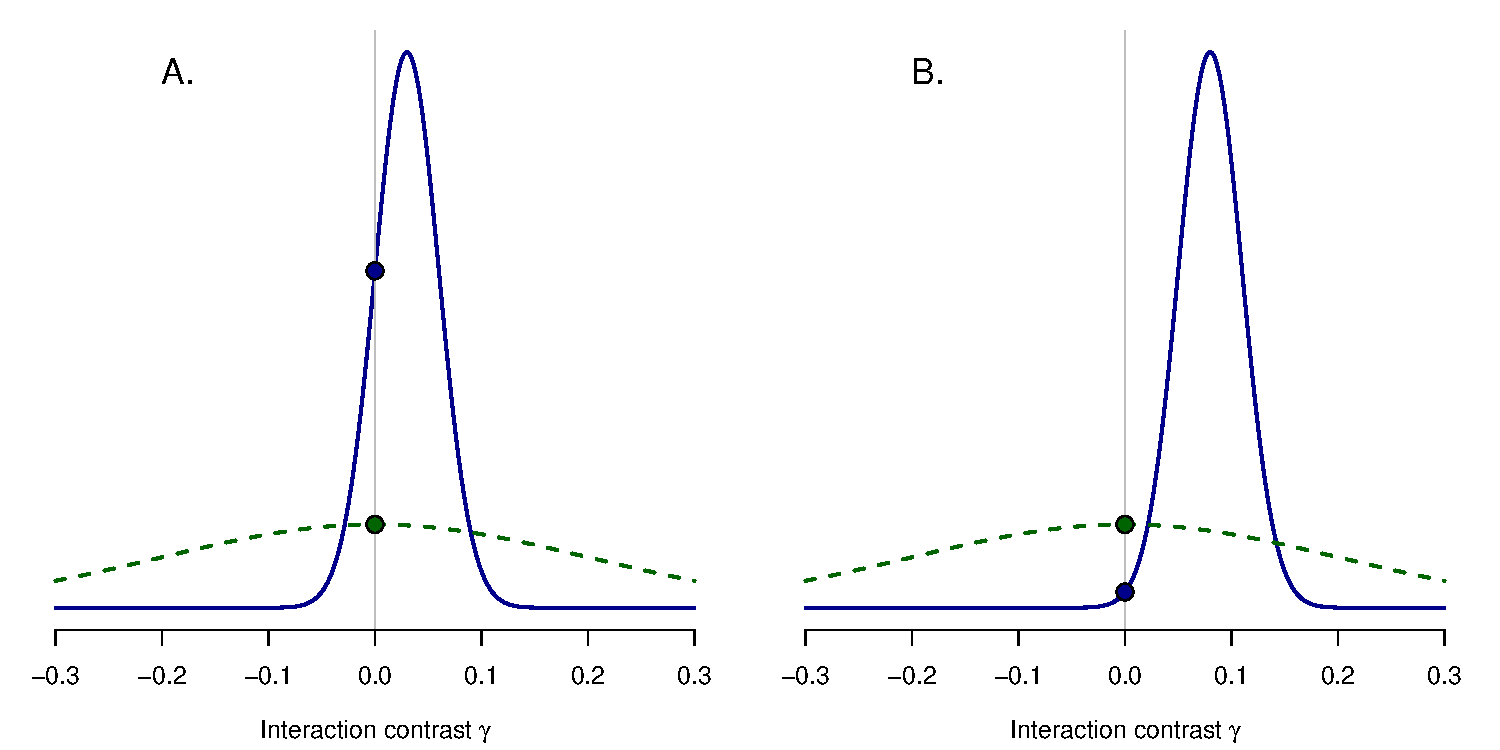
\includegraphics[width=6in]{savageDickey.pdf}
\caption{The Savage-Dickey ratio is the Bayes factor for the selected model comparisons.  Prior and posteriors are depicted  as dashed and solid lines, respectively, and the points highlight the values at zero.  {\bf A.} When the posterior is localized near zero, the posterior density at zero is higher than the prior density at zero.  {\bf B.}  When the posterior localized away from zero, the posterior density at zero is lower than the prior density at zero.}
\label{ratio}
\end{figure}


\section{Analysis}
As is common in Bayesian analysis, we use Bayes' Rule to derive conditional posterior distributions and then use Markov Chain Monte Carlo (MCMC) integration to compute marginal posterior quantities \citep{Gelman:etal:2004,Rouder:Lu:2005}.  The derivation of these conditional posterior distributions is conceptually straightforward though a tedious.  Sampling of all quantities may be done through Gibbs steps or Metropolis Hasting Steps \citep{Gelfand:Smith:1990}, and parameter blocking \citep{Roberts:Sahu:1997} speeds convergence.  The derivation of all quantities and the details of implementation may be found in \citet{Thiele:2015}.


\section{Experiment~1}
In Experiment~1 we assessed whether chunking affected processing by
comparing model outputs in a perceptual condition to those in a
working-memory condition.  In the perceptual condition, participants
were presented two screwhead stimuli that may vary
in the size of the screw and the orientation of the slot (see Figure~\ref{paradigm}).  They had to
decide if both dimensions differed or if at least one dimension was
the same.  The working memory task consisted of the same stimuli, but
instead of comparing two simultaneously presented screwheads, participants compared a presented screwhead to one presented a second previously and available only from memory.

\subsection{Method}

\subsubsection{Participants} A total of 64 participants performed in Experiment 1.  Two were discarded with one for below-chance performance and another for excessively long response times that averaged over 5 seconds.  

\subsubsection{Stimuli \& Design} Stimuli were pairs of screwheads that varied in two features: size and orientation.   Each feature could either be the same, differ by a small amount, or differ by a large amount.  Crossing these three levels yields nine possible combinations as shown in Table~\ref{task}.   

In the perception condition, screwheads were presented in white on a black background.  The screwhead on the left served as the standard.  It had  a radius that varied between 54 and 180 pixels (chosen randomly from a uniform distribution) and had an orientation that varied across all possible angles (again, chosen randomly from a uniform distribution).  The screwhead on the right had either the same size radius (no change) ,a radius that was 15 percent larger or smaller (small change) or a radius that was 30 percent larger or smaller (large change).  Likewise the screwhead on the right  had either the same orientation, a  $\pm20^\circ$ orientation difference (small change) or a $\pm60^\circ$ orientation difference (large change).  Changes in size were equally likely to be an enlargement or a reduction in radius; changes in orientation were equally likely to be clockwise or counterclockwise in direction.  


In the memory condition, screwheads were white presented on a grey background, and this change of background was needed to reduce the formation of after images of the first stimulus.  Unfortunately, our pilot participants were unable to perform the memory task at sufficiently high performance with the above changes.  To provide for high accuracy,  we increased the differences in features across the stimuli for this condition.  The radius changes were 30 and 50 percent of the original size and the orientation changes were 35 or 75 degrees of difference.  

Task condition, whether memory and perception, was manipulated in a between-subject manner with thirty and thirty-two participants performing in the memory and perception conditions, respectively.  


\subsubsection{Procedure}  A trial consisted of the events shown in Figure~\ref{paradigm}A and \ref{paradigm}B for the perception and working memory conditions, respectively.  There were 9 types of trials comprised of crossing the feature levels as shown in Table~\ref{task}.   The five negative trial types, $(0,0)$, $(0,1)$, $(0,2)$, $(1,0)$, and $(2,0)$, each occurred with probability .1.  The four positive types, $(1,1)$, $(1,2)$, $(2,1)$, and $(2,2)$ each occurred with probability .125.  There were 360 experimental trials in a session, and these were preceded by 18 practice trials.  Participants were given a pleasant doublet beep for correct responses and a less pleasant buzz for wrong ones.  Trials were blocked in groups of 60, and participants were given a self-paced break between blocks.  Trials were self paced, and participants started each by depressing a space bar.  Positive and negative responses were made by pressing the '/' and 'z' key, respectively.


\subsection{Results \& Discussion}
Figure~\ref{surf1}A-B show the empirical results for Experiment 1A, the perception condition.  At the aggregate level, there are reasonably large main effects of angle difference (.139 s) and radial size difference (.223 s).    These main effects provide some expectation that interactions, should they exist, should be on the order of .050 s or so.  Inspection of individual MICs seemingly provides support for a serial architecture for most participants.  Figure~\ref{surf1}C-D show the same for Experiment 1B, the memory condition.  The main effects of size and angle differences are a bit smaller (.047 s and .081 s for angle and size, respectively), and inspection of individual MICS in Figure~\ref{surf1}D seemingly provides similar support for the serial conclusion.

To more formally assess the evidence for various processing architectures, we fit the  six models separately for Experiment 1A and Experiment 1B.  Convergence was assessed by inspection of parameter trace plots and affirmed by comparison of posterior mean parameter estimates to observed MICs.

Parameter estimates for each $\gamma_i$, the interaction parameter, are shown as a function of observed MIC in Figure~\ref{est1}.  The estimates of $\gamma_i$ under the general model trends as the observed MIsC, and this behavior is expected as the observed MIC may be viewed as a conventional estimate of $\gamma_i$.   As can be seen, there is a much shrinkage, which is an indication that the variation in observed MICs reflects sample noise to a large extent.  The estimates for the coactivation and parallel model with individual variability (Coactive-1, Parallel-1) show expected patterns as well.  When the observed MICs are negative, the parallel model estimates tends to track well and the coactive estimates tends to track to zero as it cannot be negative.  The reverse pattern holds for positive observed MICs.  Again, there is a fair amount of shrinkage.  The two lines are the estimates for coactivetion and parallel models with no individual variability  (Coavtive-2, Parallel-2); and these both are very near zero. 

\begin{figure}
\centering
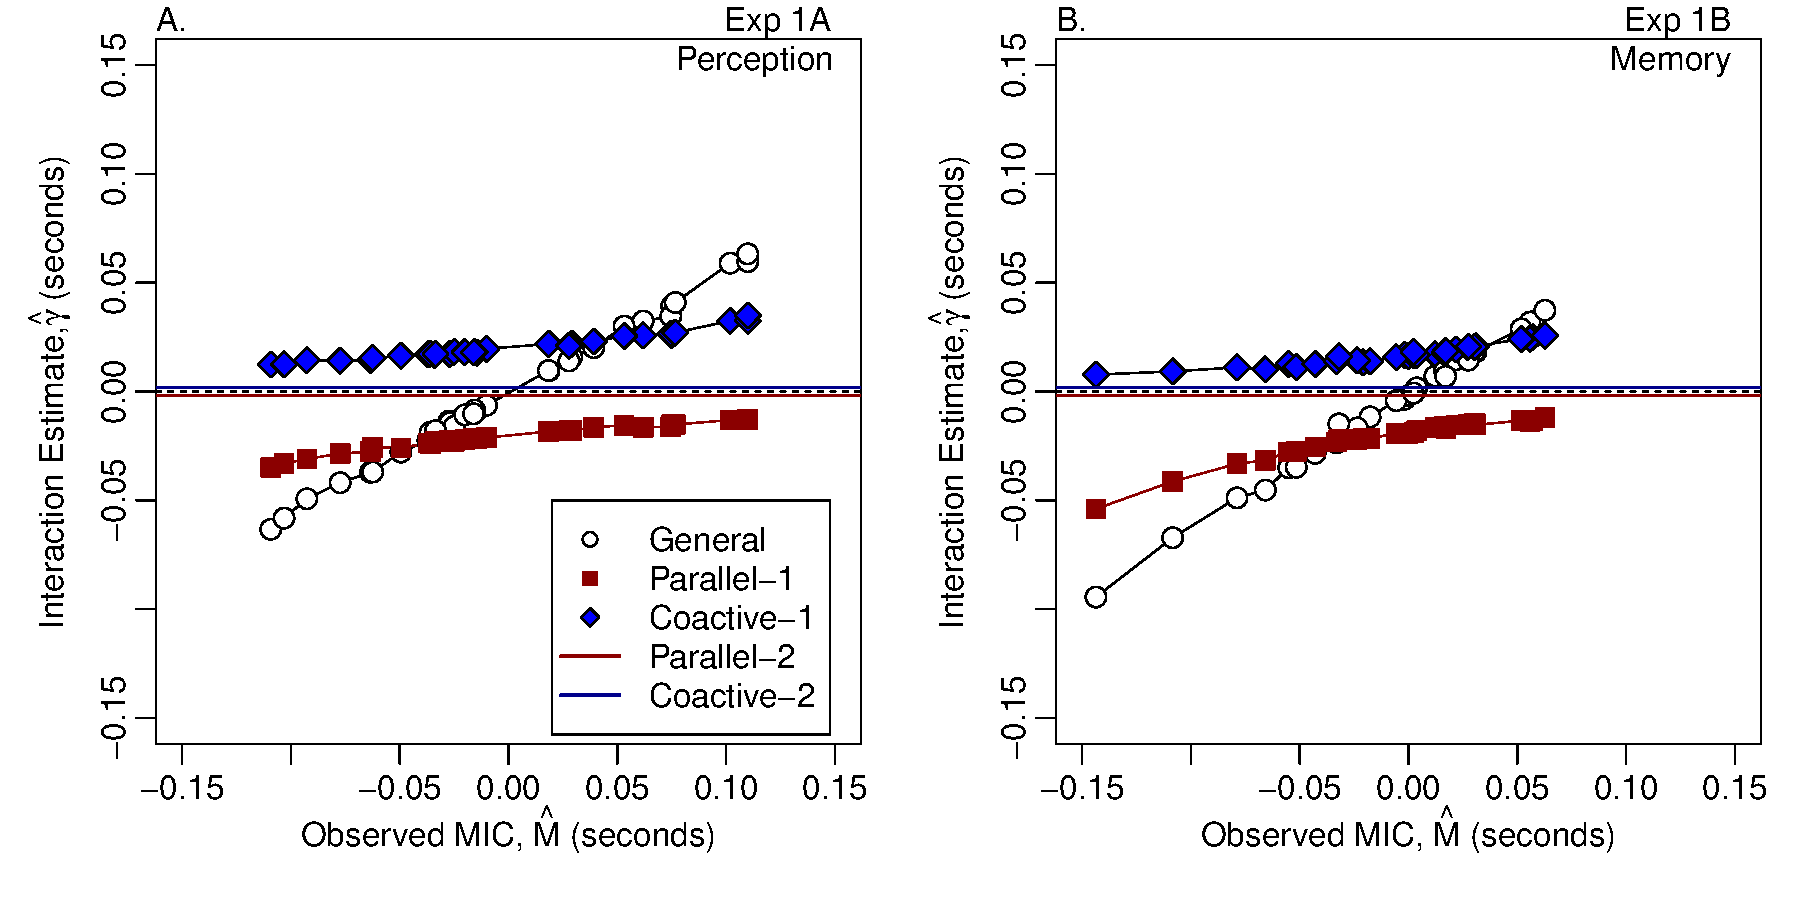
\includegraphics[width=6in]{jonFigures/jEst1.pdf}
\caption{Model-based estimates of the interaction parameter $\bfgamma$ for Experiment 1.  {\bf A.} Results for Experiment 1A, the perception experiment.  {\bf B.} Results for Experiment 1B, the memory experiment.}
\label{est1}
\end{figure}


Table~\ref{bf1} provides the Bayes factors for both perceptual and mnemonic conditions  The Bayes factor values are the strength of evidence for the serial model relative to other models.  For example, the first value in the Table, 9.0 \scN{13}, indicates that the data are almost 14 orders of magnitude more likely under the serial model than under the parallel-1 model.    Two trends are evident for both conditions: first, the serial model outperforms the others in both the perception and memory conditions.  The smallest Bayes factor is 4.4-to-1 indicating that in all conditions, the data were over 4 times more probably under the serial model than any under any competitor model.  The second trend is that the models that allowed for individual variation, the general, coactive-1, and parallel-1 models, do particularly poorly.  The associated Bayes factor is several orders of magnitude less than the models that constrain individuals to have the same true effect.  These values serve as evidence for the proposition that people do not truly vary from one another, and that the observed variation is due largely to sample noise.


\begin{table}
\caption{Bayes factor values in favor of  serial model vs. competitors \label{bf1}
}
\begin{tabular}{lcccc}
& \multicolumn{2}{c}{Experiment 1}&\multicolumn{2}{c}{Experiment 2}\\
& Perception & Memory & Perception & Memory \\ \hline
&\multicolumn{4}{c}{Normal Parametric Models}\\
Parallel-1 & 9.0 \scN{13} & 2.2 \scN{13} & 1.2 \scN{9} & 2.2 \scN{7}\\
Parallel-2 & 11.7 & 4.44 & 1.51 & .61\\
Coactive-1 & 1.1 \scN{14} & 2.4 \scN{16} & 2.5 \scN{18} & 1.0 \scN{19}\\
Coactive-2 & 13.5 & 29.7 & 47.0 & 60.6\\
General & 2.5 \scN{2} & 1.3 \scN{2} & 2.1 \scN{1} & 4.8 \scN{1}
%&\multicolumn{4}{c}{Gamma Parametric Models}\\
%Parallel-1 & 7.8 \scN{15} & 6.4 \scN{15} & 9.7 \scN{12} & 2.5 \scN{13}\\
%Parallel-2 & 12.6 & 9.34 & 4.69 & 2.69\\
%Coactive-1 & 3.5 \scN{18} & 6.1 \scN{16} & 5.3 \scN{17} & 4.0 \scN{18}\\
%Coactive-2 & 16.4 & 22.6 & 32.8& 44.5\\
%General & 2.4 \scN{6} & 2.1 \scN{7} & 2.9 \scN{7} & 3.3 \scN{7}\\ \hline
\end{tabular}
\end{table}


These results are surprising to  us.  We had expected that recall from working memory would rely on a different architecture than perception, perhaps through consolidation, grouping, or chunking.  Yet, we found both tasks were mediated by serial processing of features.  We has also expected that there might be noticeable individual differences.  These expectation were guided by previous results in systems-factorial technology where analysis of individuals, albeit as fixed effects, sometimes reveals variability in processing \citep[e.g.,][]{Little:etal:2011}, as well as by general trends in the field where individual differences are expected and interpreted.  Yet, we found evidence against individual variation in true interactions.  Models with individual variation were heavily penalized for this flexibility, and models with a single true value fared much better.  We discuss qualifications on these findings in the General Discussion.



%
%\begin{figure}
%\centering
%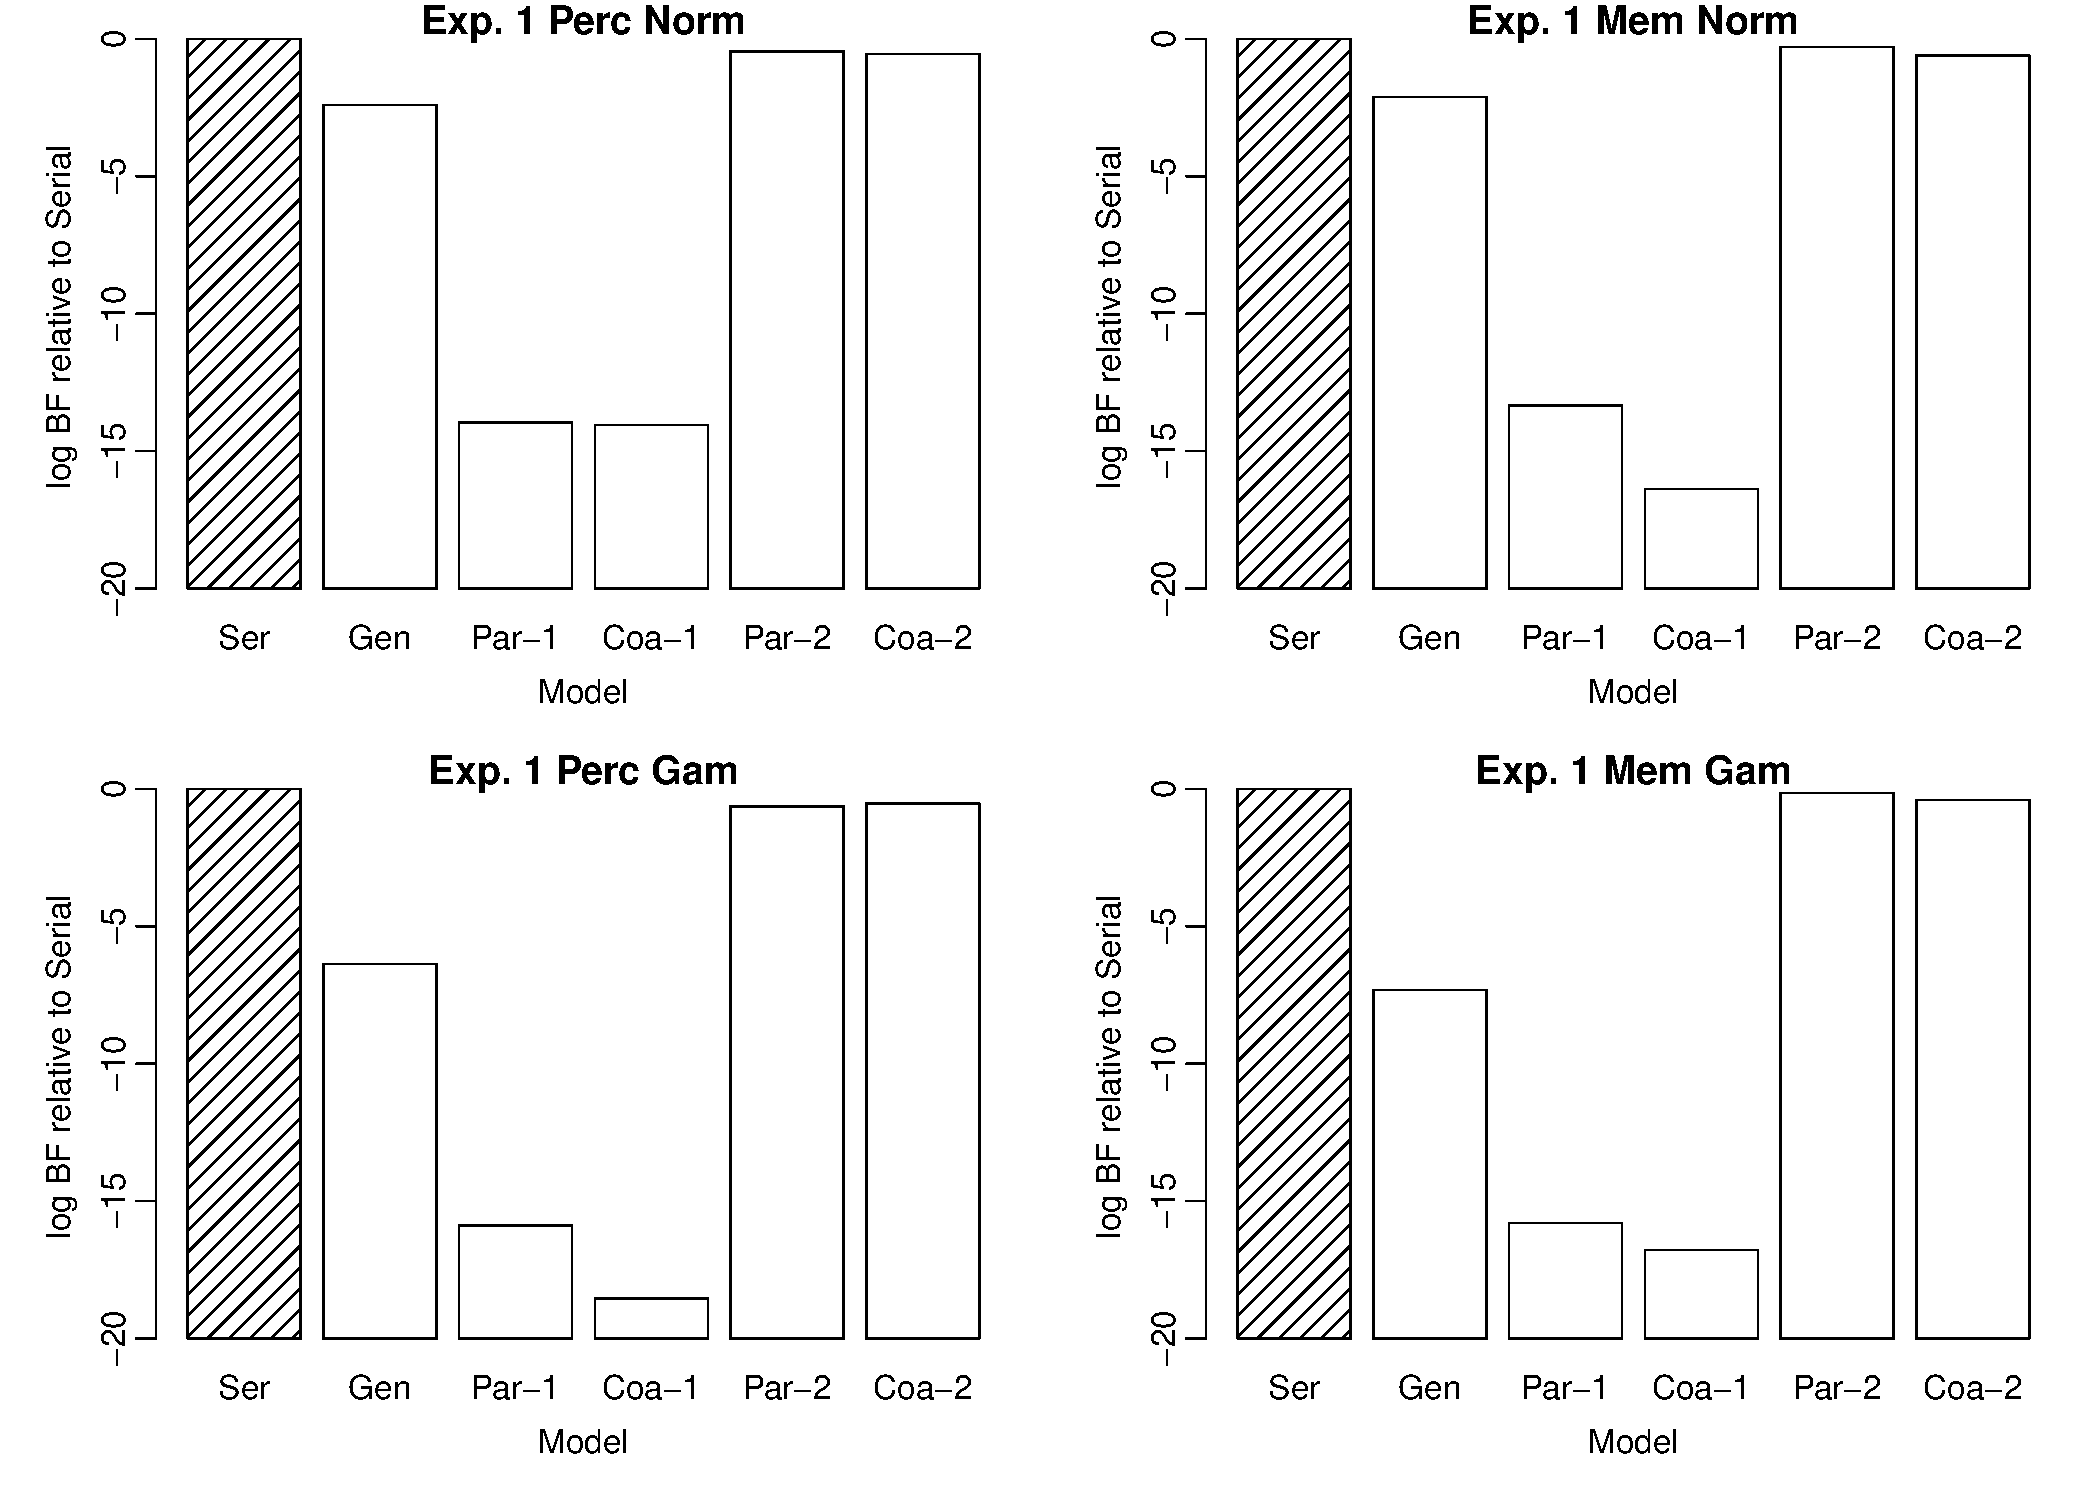
\includegraphics[width=6in]{E1BFBars.pdf}
%\caption{Bayes factor model comparison for Experiment 1.  The four panels show the crossing of the perceptual and mnemonic condition with the normal and gamma parametric forms.  The bars are Bayes factor for each model relative to the serial model.  The serial model does best in all cases, and the three models with individual variability, the general, coactive-1, and parallel-1, do particularly poorly indicating evidence against true individual variation.}
%\label{bf1}
%\end{figure}




\section{Experiment~2}
Experiment~1 revealed serial processing in both the perception and working-memory tasks.  In Experiment 2 we attempted to promote explicit chunking by using two-digit number stimuli instead of screwheads.  An example stimulus was the number  ``46."   We treat each digit is a feature, called the 10s feature and the 1s feature.  A  difference in the 10s feature is seen in the difference between the numbers ``46" and ``56"; a difference in the 1s feature is seen between the numbers ``46" and ``47"; and a difference in both features is seen between the numbers ``46" and ``57."  These differences in digits could be small, $\pm1$, as in the previous examples, or large, $\pm3$.  For example "46" and "19" differ by a large amount in both features.    Experiment 2 followed the same structure of Example 1; the main difference was the type of stimuli.

Whether the size of the change manipulation, from $\pm1$ to $\pm3$, affects responses deserves further scrutiny.   Digit change size matters if digits are processed as magnitudes that than as abstract symbols.  Evidence for magnitude processing comes from the well-known distance-from-five effect \citep{Moyer:Landauer:1967}.   Participants in the distance-from-five task must identify whether a single-digit number is less-than or greater-than five.  \citet{Rouder:etal:2005a} found that responses to digits far from five, 2 and 8, are responded to .05 s faster than digits close to five, 4 and 6.  In Experiment 2, we find similar differences across the change size manipulation as is discussed subsequently. 

\subsection{Method}
\subsubsection{Participants}  A total of 56 University of Missouri students participated in exchange for course credit.  No participants were discarded.


\subsubsection{Stimuli}  The left-hand number served as the standard, and the digits that comprised it varied between 4 and 6, inclusively.  In the small change condition, the digits of a common feature varied by $\pm1$; in the large change condition digits in the common feature varied by $\pm3$.  Changes were equally likely to be positive or negative.  The same nine combinations as Experiment~1 were used in the same frequencies.

\subsubsection{Procedure}
The procedure for Experiment 2 was identical to Experiment 1 with the exception that balanced stimulus presentations.  Of the 360 trials, there were 36 for each type of negative trial and 45 for each type of positive trial.  In Experiment 1, in contrast, we set probabilities, but the numbers of each trial type varied from participant to participant.

\subsection{Results}
Figure~\ref{surf2}A and \ref{surf2}B show the empirical results for Experiment 2A, the perception condition.  Figure~\ref{surf2}C and \ref{surf2}D show the same for Experiment 2B, the memory condition.  A critical question in whether the change-size manipulation, the difference between $\pm1$ and $\pm3$ mattered.  The effect across all conditions is about .082 s, which is reasonably large for these type of digit effects \citep{Moyer:Landauer:1967,Rouder:etal:2005a}.   Inspection also yields the possibility of an interaction where the change-size is overadditive when there is a large change in both digits.  This type of interaction corresponds to a negative MIC.   Yet, inspection of individual MICs seemingly provides support for a serial architecture for many participants.   A noteworthy minority of participants in the memory condition display patterns consistent with a negative MIC, a pattern consistent with parallel processing.

\begin{figure}
\centering
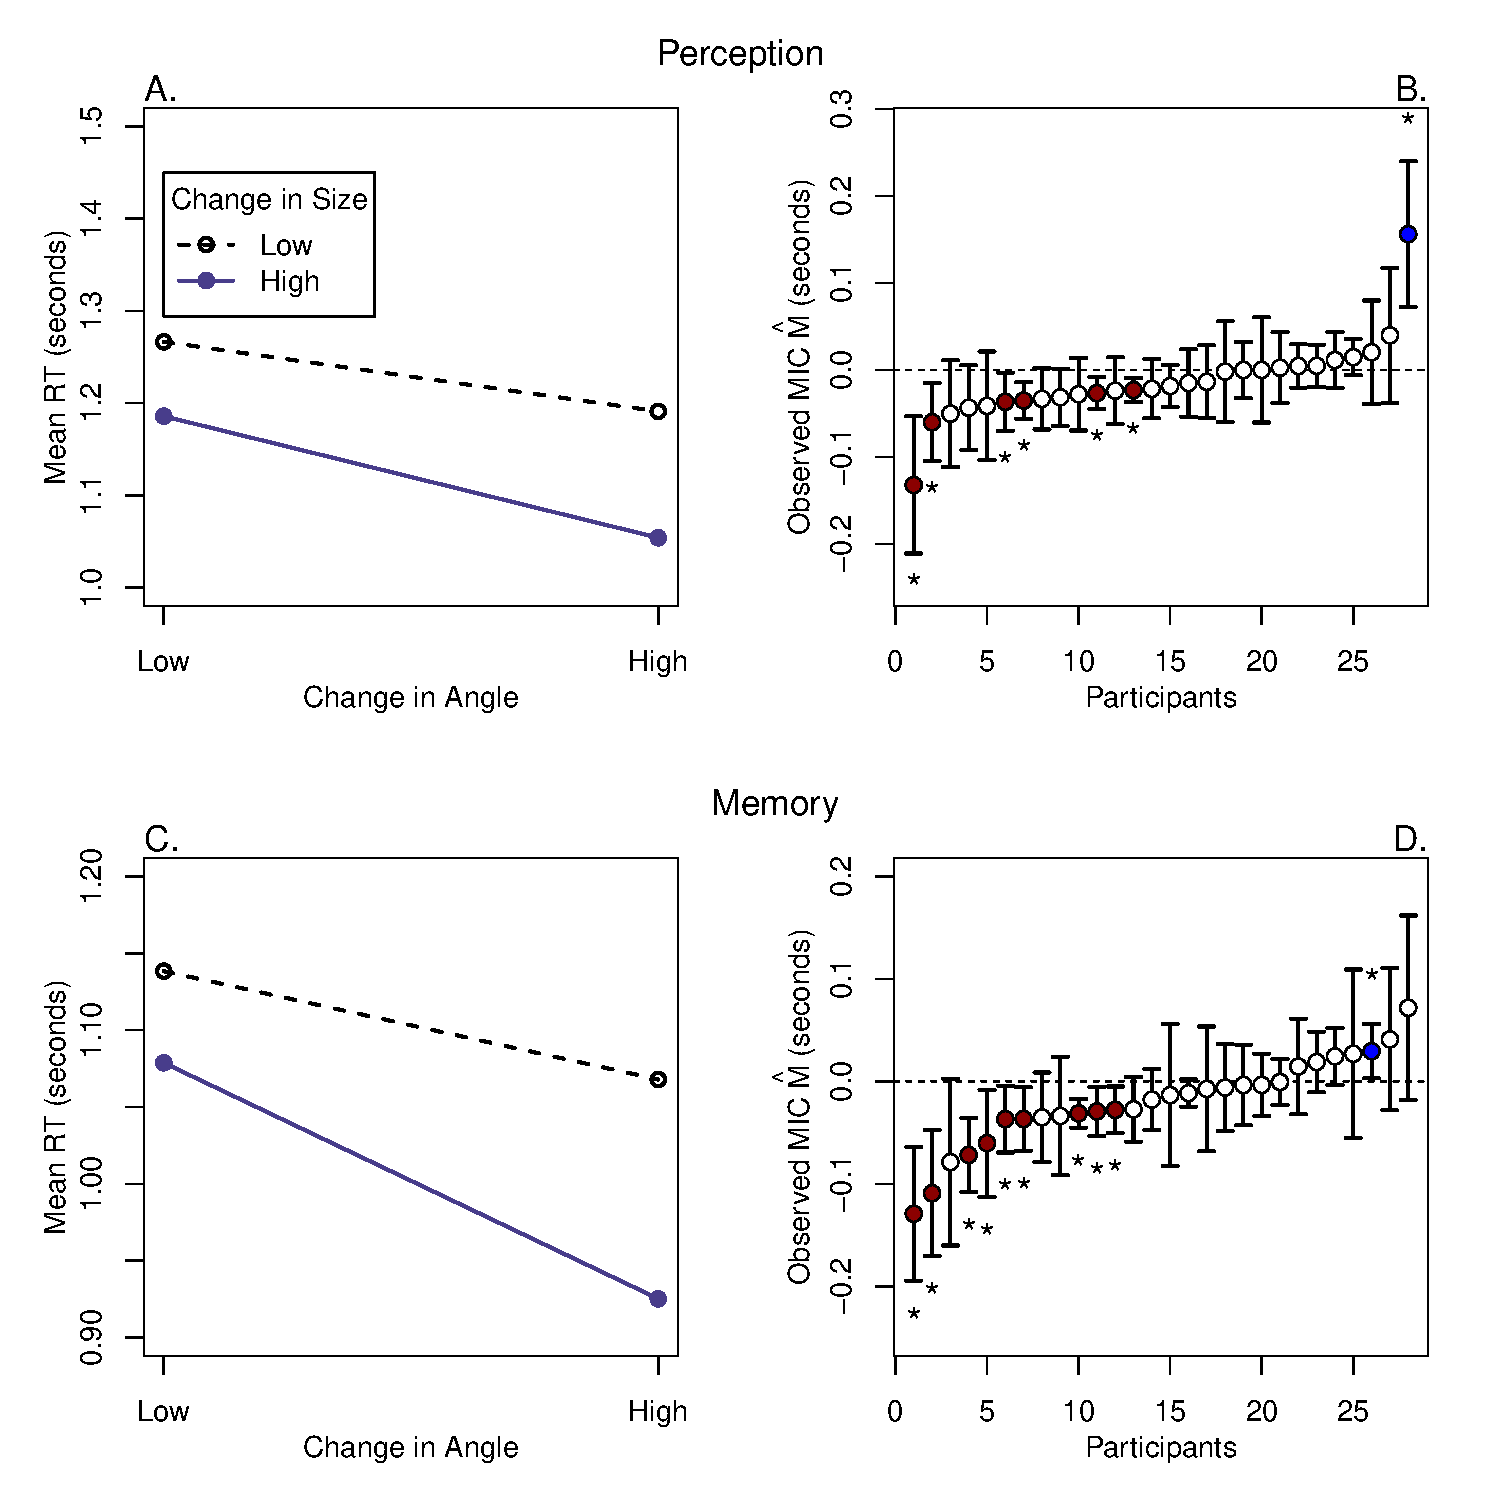
\includegraphics[width=6in]{jonFigures/jE2.pdf}
\caption{Results from Experiment 2:  {\bf A.,C.} Observed mean response times for Experiments 1A (perception) and 1B (memory), respectively.  {\bf B., D.} Observed mean interaction contrasts (MICs) with 80\% confidence intervals for each if 31 individuals.  The CIs with open circles contain zero (serial processing); those with darkened circles and an asterisk below are all negative (parallel processing); those with darkened circles and an asterisk above are all positive (coactive processing).}
\label{surf2}
\end{figure}

Parameter estimates for each $\gamma_i$, the interaction parameter is shown as a function of observed MIC in Figure~\ref{est2} and the patterns are comparable to Experiment~1.  The Bayes factors are shown in Table~\ref{bf1}.  Some trends are the same as in Experiment 1 including the dramatic advantage for single-effect models (serial, parallel-1, and coactive-1) over models that allow for different effects for each participant.  Also, like in Experiment 1, the serial model did well at least in the perception condition.  Yet, the evidence comparing the serial model to single-effect parallel model is not overly convincing---the Bayes factors is 1.5 in favor serial model.  The case is even more ambiguous for the memory condition.  Here, the evidence slightly favors the parallel model.   We think it is judicious to be cautious and hold skepticism from the small magnitude of these Bayes factors.  Rather than split hairs about specification, we suspect a more clear evidence would come from an improved experiment.  Future work should focus on improving the design, perhaps by loading memory with more than one item (though it is not clear that this may be done while retaining high accuracy needed for the analysis).

\begin{figure}
\centering
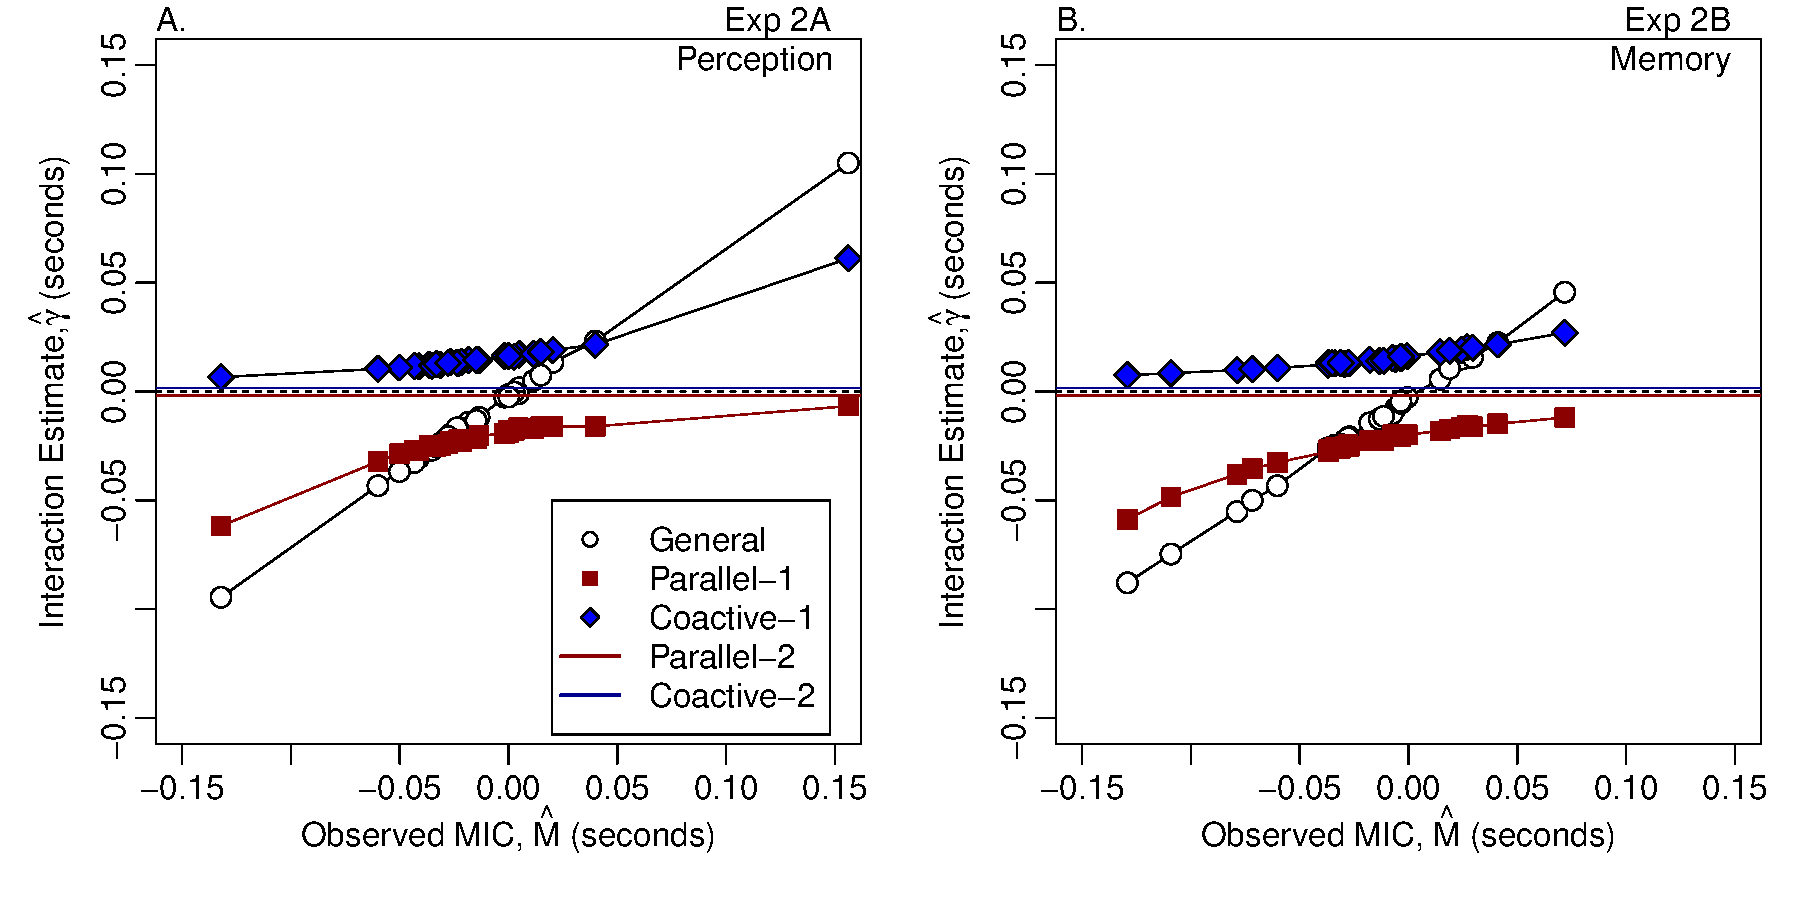
\includegraphics[width=6in]{jonFigures/jEst2.pdf}
\caption{Model-based estimates of the interaction parameter $\bfgamma$ for Experiment 2.  {\bf A.} Results for Experiment 1A, the perception experiment.  {\bf B.} Results for Experiment 1B, the memory experiment.}
\label{est2}
\end{figure}




\section{General Discussion}
Systems factorial technology is an exciting methodology for addressing fundamental questions about processing architecture.  We address some of the real-world statistical difficulties in analysis including the lack of common-architecture models across individuals.  We propose six substantive models that address whether processing is serial, parallel, or coactive, and whether there is truly individual variation or not.  Comparisons among these models may be made with Bayes factors, and these ratios serve as principled relative evidence among the models.   We hope the model-comparison methods developed here may be broadly applicable to system-factorial applications.

We applied the Bayes factor model comparison methods to understand whether chunking in working memory changes the architecture of processing.  Our experiments consisted of a perceptual and mnemonic conditions, and it was expected that this change in task would perhaps be associated with a change in processing.  Plausibly, the chunking in working memory could have consolidated the features into a single whole that could be processed more efficiently than serially.  These results, however, were not observed.  The evidence from Bayes factors favored the serial model in almost all cases indicating that features were compared in a serial fashion for both perceptual and mnemonic tasks.  This evidence, however, is scant  in the numbers task where the single-effect parallel model is a plausible contender.  In summary, there is no evidence for any change in architecture with chunking.

We are unsure whether these findings places constraints on theories of working memory.  Perhaps the serial finding reflect task demands that may not be present in other working-memory paradigms.  In this paradigm, participants are asked to decide whether both features have changed or, alternatively, one or fewer features had changed.  The task may require that even if the stimuli are chunked together for storage purposes, they may be split into separate features to make the task-relevant response.    If this is the case, then it is hard to see how the finding constrains theories of working memory; instead it constrains theories of how this task is performed at least for these stimuli.  Additionally, we are concerned about the ambiguous evidence from the number stimuli, and suspect that loading memory with more than one item might yield more discriminative results.  Clearly, more work needs to be done.

The dramatically poor performance of models that ascribe true individual differences to participants was unexpected.  It is nearly ubiquitous that individual variation is reported and expected across most tasks of human performance.  Yet, we found strong evidence against such individual variation in the interaction parameter.    The case is similar to our previous findings with reading speeds.  \citet{Rouder:etal:2008d} provided a hierarchical Bayesian analysis of how lexical decision times varied with word frequency.  The found that once shift latencies from motor and encoding stages were subtracted, all individuals had the same 11\% decline per doubling of word frequency.  There was no evidence of deviation from this 11\% value across the 50 participants.

Some readers may find it difficult to believe models without true individual variation.    It is important to keep in mind that models are just abstractions that vary is usefulness across contexts.   No model is true or false; in fact, it is misguided to ascribe truth values to models at all \citep{deFinetti:1974,Morey:etal:2013}.  The constant models without individual variation are probably good models when the sample sizes (trials per participant) are not too large.  For the resolution afforded by the data in hand, there is no need to consider individual variation.  However, it may be the case with larger sample sizes, that models with individual variation is warranted.  In this spirit, we recommend that models with constant effects be retained and taken seriously because at a minimum because they indicate whether the data are sufficiently numerous to resolve individual variation.   In this case, they do not provide such resolution.  With the insights from Bayesian model comparison herein and previously, we recommend that those who advocate individual variation in performance document this variation with the proper and principled comparison of hierarchical models.  We suspect it will be harder to provide this documentation than commonly assumed as it requires data with large sample sizes per participant.  And this last point, if taken seriously, may be the most disruptive insight from this report.

\clearpage
\bibliography{lab}

\clearpage
\section{Appendix}

Prior specification is needed for $\sigma^2$, the common variance, and for vectors $\bfeta$, $\bfalpha$ and $\bfbeta$.  The prior on $\sigma^2$ is $\sigma^2 \sim \mbox{Inverse Gamma} \left(2,\frac{1}{4}\right)$.   The induced prior on standard deviation has sizable mass above 180 ms, peaks at about 400 ms, and slowly tails off with a fat tail that allows standard deviations as large as 2 seconds.  This prior though informative is sufficiently broad for response times in simple tasks such as those reported here.

The remaining parameters are individual-specific effects, and we chose to model them as  unconstrained random effects with a hierarchical structure:
\begin{eqa*}
\eta_i &\sim& \mbox{Normal}\left(\nu_{1},\delta_{1}\right),\\
\alpha_i &\sim& \mbox{Normal}\left(\nu_{2},\delta_{2}\right),\\
\beta_i &\sim& \mbox{Normal}\left(\nu_{3},\delta_{3}\right),
\end{eqa*}
where $\nu$ and $\delta$ are respective group mean and variances.  Priors on the group mean parameters are
\[
\nu_{1} \sim \mbox{Normal}(2,1),\quad
\nu_{2} \sim \mbox{Normal}\left(0,.032^2\right),\quad 
\nu_{3} \sim \mbox{Normal}\left(0,.032^2\right).
\]

The scale on main effects are tuned, but are reasonable for the size of effects in cognitive psychology.
The priors on the group variance parameters are 
\[
\delta_{k} \sim \mbox{Inverse-Gamma}\left(3,\frac{1}{5}\right), \quad k=1,2,3.
\]

\end{document}


\end{document}
